\subsection{Directed Max flow}
\subsubsection{Edmonds-Karps (BFS)}
Path in residual graph searched via BFS. $O(|V||E|^2)$.\\
\lstinputlisting{Graphs/edmondskarps.java}
\subsubsection{Ford-Fulkerson}
Equals to Edmonds-Karps, but with a DFS. $O(|E|f^*)=O(|V||E|^2)$ where $f^*$ is the value of the max flow.
\lstinputlisting{Graphs/fordfulkerson.java}
\subsubsection{Min cut}
We search, between two nodes $s$ and $t$, subsets of nodes $V_1$ and $V_2$ so as $s\in V_1$, $t\in V_2$ and $\sum_{e \in E(V_1, V_2)} w(e)$ minimum.\\
We just have to compute the max-flow between $s$ and $t$ and to apply a BFS/DFS on the residual graph. All node which are visited are in $V_1$, others in $V_2$. The weight from the cut is the max-flow.
\subsubsection{Maximum number of disjoint paths} 
For edge disjoint paths just compute the max flow with unit capacities. For vertex disjoint paths split vertices into two with unit capacity edge between them.
\subsubsection{Maximum weighted bipartite matching}
Assignment problem: Given a set of $n$ persons and $n$ jobs, and a cost matrix $M$, assign a job to each person such that the sum of the costs is minimized. It also works for $n$ persons and $m$ jobs with $n \neq m$. Just fill make a square matrix using dummy values. Can also be solve with min cost max flow but it is slower. \\

$O(n^3)$ solution:
\lstinputlisting{Graphs/mwbm.java}
\vspace{0.5cm}
$O(n 2^n)$ solution using DP (very simple to code):
\lstinputlisting{Graphs/mwbmDP.java}

\subsection{Directed Min cost flow}
Avoiding parallel edges:
\begin{enumerate}
\item Split nodes
\begin{center}
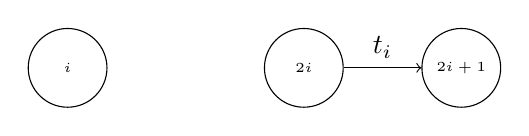
\begin{tikzpicture}
\node[draw, circle, minimum size = 1cm] (i) at (0, 0) {\tiny $i$};
\node[draw, circle, minimum size = 1cm] (i1) at (3, 0) {\tiny $2i$};
\node[draw, circle, minimum size = 1cm] (i2) at (5, 0) {\tiny $2i + 1$};
\path[->] (i1) edge node[anchor=south] {$t_i$} (i2);
\end{tikzpicture}
\end{center}
where $t_i$ is the number of times node $i$ can be used (usually $\infty$).\\

\item Link nodes
\begin{center}
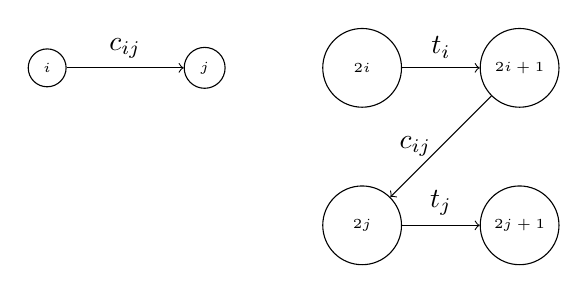
\begin{tikzpicture}
\node[draw, circle] (i) at (-1, 0) {\tiny $i$};
\node[draw, circle] (j) at (1, 0) {\tiny $j$};
\path[->] (i) edge node[anchor=south] {$c_{ij}$} (j);
\node[draw, circle, minimum size = 1cm] (i1) at (3, 0) {\tiny $2i$};
\node[draw, circle, minimum size = 1cm] (i2) at (5, 0) {\tiny $2i + 1$};
\node[draw, circle, minimum size = 1cm] (j1) at (3, -2) {\tiny $2j$};
\node[draw, circle, minimum size = 1cm] (j2) at (5, -2) {\tiny $2j + 1$};
\path[->] (i1) edge node[anchor=south] {$t_i$} (i2);
\path[->] (j1) edge node[anchor=south] {$t_j$} (j2);
\path[->] (i2) edge node[anchor=east] {$c_{ij}$} (j1);
\end{tikzpicture}
\end{center}
\end{enumerate}

\lstinputlisting{Graphs/transform.java}

Min cost flow analogous to max flow but using Bellman-Ford to find paths (can be made faster using Dijkstra by chaining costs).\\

\lstinputlisting{Graphs/mincostflow.java}

Some changes to SPFA may be necessary. Computation of global variable $p$ containing parents is required.

\subsection{Chinese Postman Problem}

Given an undirected weighted graph, compute the minimum length tour that visits every edge (edges may be visited several times, unavoidable if odd degree vertices exist). The number of odd degree vertices is even. Hence we can compute the minimum weight bipartite matching between them where $w_{ij}$ is the length of the shortest path between $i$ and $j$. Then the length of the tour is given by the sum of the lengths of all edges plus the weight of the matching.